\section{Laboratory work implementation}

\subsection{Tasks and Points}

\begin{itemize}
	\item Crearea unui friendly UI pentru calculator
	\item Supraincărcarea unui Tool implicit pentru lucrul cu stringurile intr-un calculator
	\item Crearea funcționalității elementare de lucru cu UI
	\item Adăugarea modulului Core pentru calculele necesare unui calculator
	\item Adăugarea funcționalitatea pentru urmatoarele functii: +, -, /, *, putere, radical, InversareSemn(+/-), operatii cu numere zecimale
	\item Bug fixing
\end{itemize}

\subsection{Analiza lucrarii de laborator}
Repository \href{https://github.com/AScripnic/MIDPS-laboratories/tree/master/Lab%232}{link}\par

Primul pas făcut în crearea calculatorului a fost UI-ul și definirea fiecărui buton de care am avut nevoie în acest proiect. După adăugarea butoanelor, am schimbat toate denumirile implicite \hl{buttonNo} în unul mai potrivit \hl{devideButton}. \par

Pentru un lucru mai ușor cu label-ul care afișează valoarea curentă am supraîncărcat in tool-ul \href{https://github.com/AScripnic/MIDPS-laboratories/blob/master/Lab%232/Core/Core/ExtendedLabel.cs}{label} în care am inclus unele metode care mau ajutat să lucrez mai ușor cu string-urile. \par

Am creat \href{https://github.com/AScripnic/MIDPS-laboratories/blob/master/Lab%232/Calculator/Calculator/Form1.cs}{metodele} pentru fiecare acțiune generata din UI, de exemplu:
\begin{itemize}
	\item Adăguarea unei noi cifre la ecran
	\item Ștergerea unei cifre
	\item Adăugarea, împărțirea, radical, puterea
	\item Etc.
\end{itemize}

Pentru calculele matematice am creat un module nou \href{https://github.com/AScripnic/MIDPS-laboratories/tree/master/Lab%232/Core/Core}{Core}, in care se fac toate operatiile de calcul si de stocare a rezultatelor.
In acest modul se pastrează ultimul semn accesat si ultima valoare scrisă cu scopul de a afișa îndată rezultatul cerut. \par

Unul din cele mai importante buguri întalnite a fost \href{https://github.com/AScripnic/MIDPS-laboratories/blob/master/Lab%232/Calculator/Calculator/Form1.cs#L74}{depăsirea numărului maxim disponibil} tipului de date double \cite{bugs}:.


\subsection{Imagini}
\begin{center}
	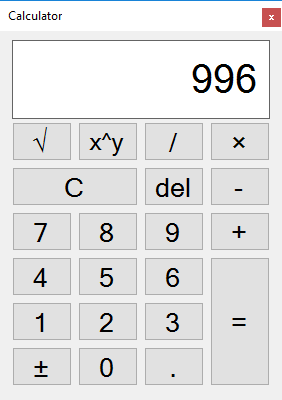
\includegraphics[scale=0.8]{calculator}\\
	Figura 1. Calculatorul

	\bigskip 
	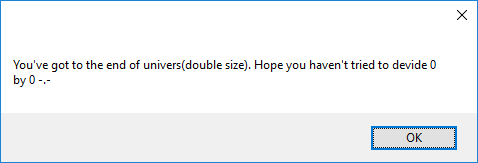
\includegraphics[scale=0.8]{infinit}\\
	Figura 2. Mesajul de atentionare
\end{center}

\clearpage